\documentclass[12pt]{article}
\usepackage{fancyhdr}
\pagestyle{fancy}
\fancyhf{}
\fancyfoot[C]{\thepage}
\fancyfoot[L]{\scriptsize CC BY-NC-SA 4.0 \textbullet\ Leo Liang}
\renewcommand{\headrulewidth}{0pt}
\usepackage[margin=1in]{geometry}
\usepackage{amsmath, amssymb}
\usepackage{array, booktabs}
\usepackage{pgffor}
\usepackage{tikz}
\parindent=0pt
\parskip=1em
\newcolumntype{C}[1]{>{\centering\arraybackslash}p{#1}}
\newcommand{\wl}{\par\vspace{5mm}\noindent\rule{\linewidth}{0.4pt}\par\vspace{1mm}}
\newcommand{\wls}[1]{\foreach \i in {1,...,#1}{\wl}}
% ─────────────────────────────────────────────────────────────────────────────
\begin{document}
\pagestyle{fancy}
\begin{center}
  {\Large\bfseries Homework 9}\\[4pt]
  Limits at Infinity: Two Ways\\[6pt]
  Name:\;\underline{\hspace{6.5cm}}\quad
\end{center}
\hrule\bigskip

\section*{Instructions}
Use a \textbf{pen} and \textbf{show every step}. \textcolor{blue}{Read through the readings slowly and ensure you understand \textbf{everything}}. Take your time and do not rush, it will only hurt you later. Take notes in your notebook of important information that you learn on here. This homework solves \emph{one} limit two different ways --- first
by a quick intuition, then rigorously with the limit laws --- so you can see that a good shortcut and careful
algebra give the same answer. Read each section before its problems. You may use the internet + AI as a \textbf{teacher}, but do each problem yourself first and only use it once you fail.

% ===========================================================================
\section*{The running example}
Throughout this homework we will keep returning to one limit:
\[
  \lim_{x \to \infty} \frac{2x^2 + 3x - 1}{4x^2 - x + 5}.
\]
Section 1 finds it in three lines by intuition. Section 2 finds it again, slowly and rigorously. Both should land
on the same number.

% ===========================================================================
\section*{Section 1 --- Dropping the Lower-Order Terms}

\subsection*{Reading --- why the biggest term wins}
When $x$ is enormous, not all terms matter equally. Let's start with some intuition: suppose we have the expression $x+1$. When $x$ is a large number like $1{,}000$ we have 
\[
    x + 1 = 1000 + 1 = 1001.
\]
Notice how the constant $1$ contributed barely anything to our final value $1001$. You can imagine as $x$ gets really large like $1{,}000{,}000$ the constant $1$ does even less. So we can say mathematically, for large values of $x$,
\[
    x + 1 \approx x.
\]
Now lets compare $x^2$ and $x$ at $x = 1{,}000{,}000$:
\[
  x^2 = 1{,}000{,}000 \times 1{,}000{,}000 = 1{,}000{,}000{,}000{,}000, \qquad x = 1{,}000{,}000.
\]
The $x^2$ term is a \textbf{million times larger} than $x$. The behavior you saw for the expression $x + 1$ also holds for variables. That is, for really large values of $x$, 
\[
    x^2 + x \approx x^2
\]
Now looking at the expression $2x^2 + 3x - 1$, the $+3x$ and $-1$ terms are like fleas riding on an
elephant --- they are there, but they do not move the total in any noticeable way. So as $x \to \infty$,
\[
  2x^2 + 3x - 1 \;\approx\; 2x^2, \qquad 4x^2 - x + 5 \;\approx\; 4x^2.
\]
The \textbf{highest-power term dominates}. Keeping only those dominant terms:
\[
  \lim_{x \to \infty} \frac{2x^2 + 3x - 1}{4x^2 - x + 5}
  \;\approx\; \lim_{x \to \infty} \frac{2x^2}{4x^2}
  \;=\; \lim_{x \to \infty} \frac{2}{4}
  \;=\; \frac{2}{4} \;=\; \frac{1}{2}.
\]

\subsection*{The picture}
Here is the graph of that function $f(x) = \dfrac{2x^2 + 3x - 1}{4x^2 - x + 5}$. Notice how, far out to the right, the curve flattens toward
the dashed line $y = \tfrac{1}{2}$ --- that horizontal line is exactly what ``the limit at infinity is $\tfrac12$''
means.

\begin{center}
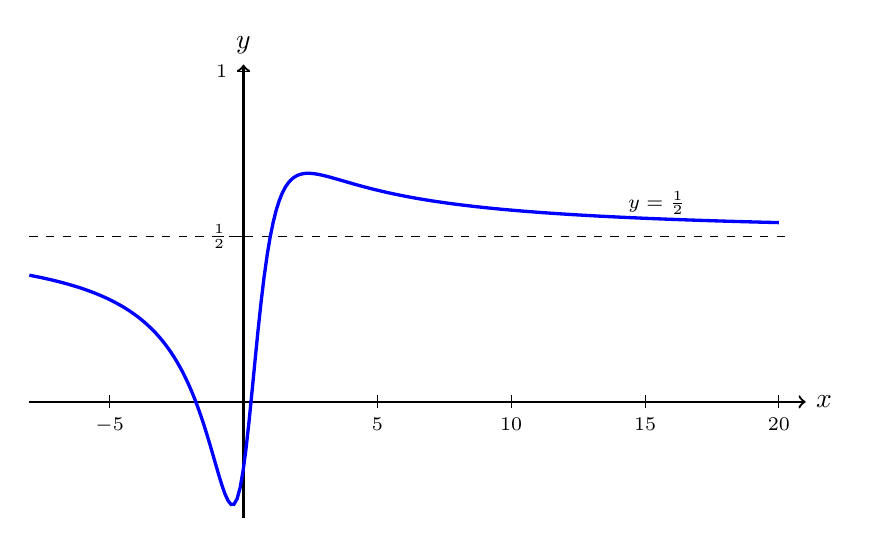
\begin{tikzpicture}[xscale=0.34, yscale=4.2]
  % axes
  \draw[thick,->] (-8,0)--(21,0) node[right]{$x$};
  \draw[thick,->] (0,-0.35)--(0,1.02) node[above]{$y$};
  % x ticks
  \foreach \tx in {-5,5,10,15,20}{\draw (\tx,0.02)--(\tx,-0.02) node[below]{\scriptsize$\tx$};}
  % y ticks
  \draw (0.25,0.5)--(-0.25,0.5) node[left]{\scriptsize$\tfrac12$};
  \draw (0.25,1)--(-0.25,1) node[left]{\scriptsize$1$};
  % horizontal asymptote
  \draw[dashed] (-8,0.5)--(20.5,0.5);
  \node[anchor=west] at (14,0.6) {\scriptsize$y=\tfrac12$};
  % the curve
  \draw[very thick,blue,domain=-8:20,samples=250] plot(\x,{(2*\x*\x+3*\x-1)/(4*\x*\x-\x+5)});
\end{tikzpicture}
\end{center}

\newpage
\subsection*{Three possible outcomes}
When dealing with a ratio of polynomials, comparing the dominant terms tells you which of three things will happen \textcolor{blue}{(ask yourself: do you know what a ``\textit{ratio of polynomials}" is? if not, search it up!)}:
\begin{enumerate}
  \item \textbf{Same degree (numerator and denominator):} the limit is the ratio of the leading coefficients
        (our example: $\tfrac{2}{4} = \tfrac12$).
  \item \textbf{Degree of the denominator is greater:} the denominator grows faster, so the fraction is crushed to
        $\mathbf{0}$.
  \item \textbf{Degree of the numerator is greater:} the numerator grows faster, so the fraction blows up to
        $\boldsymbol{\pm\infty}$ (no finite limit).
\end{enumerate}
\textcolor{blue}{(ask yourself: do you know what a ``\textit{degree}" is? if not, you could not have understood the three bullet points above. search it up!)}

\subsection*{Problems --- use the dominant-term shortcut}
For each, state which of the three cases it is (1, 2, or 3), then give the limit.

\medskip
\textbf{1.}\quad $\displaystyle\lim_{x \to \infty} \frac{5x^3 + 2x}{x^3 - 7}$
\wl

\textbf{2.}\quad $\displaystyle\lim_{x \to \infty} \frac{3x + 4}{x^2 + 1}$
\wl

\textbf{3.}\quad $\displaystyle\lim_{x \to \infty} \frac{x^2 - 6}{2x + 3}$
\wl

\textbf{4.}\quad $\displaystyle\lim_{x \to \infty} \frac{7x^2 - x}{3x^2 + 2x - 8}$
\wl

% ===========================================================================
\newpage
\section*{Section 2 --- Limit Properties and Algebra}

\subsection*{Reading --- the limit laws}
The shortcut in Section 1 works because of a few precise rules. Suppose $\displaystyle\lim_{x\to\infty} f(x)$ and
$\displaystyle\lim_{x\to\infty} g(x)$ both exist. Then:

\medskip
\renewcommand{\arraystretch}{1.5}
\begin{tabular}{@{}p{5.3cm}p{9.5cm}@{}}
\textbf{Constant Law} & $\displaystyle\lim c = c$ \\
\textbf{Sum Law} & $\displaystyle\lim \big(f + g\big) = \lim f + \lim g$ \\
\textbf{Difference Law} & $\displaystyle\lim \big(f - g\big) = \lim f - \lim g$ \\
\textbf{Constant Multiple Law} & $\displaystyle\lim \big(c\,f\big) = c \lim f$ \\
\textbf{Product Law} & $\displaystyle\lim \big(f\,g\big) = \lim f \cdot \lim g$ \\
\textbf{Quotient Law} & $\displaystyle\lim \frac{f}{g} = \frac{\lim f}{\lim g}$ \quad (provided $\lim g \neq 0$) \\
\end{tabular}
\renewcommand{\arraystretch}{1}

\medskip
And the single fact that powers this whole topic --- the one that makes ``infinity'' do useful work:
\[
  \boxed{\;\lim_{x \to \infty} \frac{1}{x^n} = 0 \quad \text{for any } n > 0.\;}
\]
As $x$ grows without bound, $\tfrac1x$, $\tfrac{1}{x^2}$, $\tfrac{1}{x^3}, \dots$ all shrink to $0$. This is the
tool that lets the algebra finish.

\newpage
\subsection*{Worked example --- the same limit, done rigorously}
We evaluate $\displaystyle\lim_{x \to \infty} \frac{2x^2 + 3x - 1}{4x^2 - x + 5}$ again. The trick: \textbf{divide
every term, top and bottom, by the highest power present} --- here $x^2$.
\[
  \frac{2x^2 + 3x - 1}{4x^2 - x + 5}
  = \frac{\dfrac{2x^2}{x^2} + \dfrac{3x}{x^2} - \dfrac{1}{x^2}}
         {\dfrac{4x^2}{x^2} - \dfrac{x}{x^2} + \dfrac{5}{x^2}}
  = \frac{2 + \dfrac{3}{x} - \dfrac{1}{x^2}}{4 - \dfrac{1}{x} + \dfrac{5}{x^2}}.
\]
Now apply the limit laws \textbf{one step at a time}, naming each one:
\begin{align*}
\lim_{x\to\infty}\frac{2+\dfrac{3}{x}-\dfrac{1}{x^2}}{\,4-\dfrac{1}{x}+\dfrac{5}{x^2}\,}
  &= \frac{\displaystyle\lim_{x\to\infty}\!\left(2+\tfrac{3}{x}-\tfrac{1}{x^2}\right)}
          {\displaystyle\lim_{x\to\infty}\!\left(4-\tfrac{1}{x}+\tfrac{5}{x^2}\right)}
     && \text{(Quotient Law)} \\[12pt]
  &= \frac{\displaystyle\lim_{x\to\infty}2+\lim_{x\to\infty}\tfrac{3}{x}-\lim_{x\to\infty}\tfrac{1}{x^2}}
          {\displaystyle\lim_{x\to\infty}4-\lim_{x\to\infty}\tfrac{1}{x}+\lim_{x\to\infty}\tfrac{5}{x^2}}
     && \text{(Sum \& Difference Laws)} \\[12pt]
  &= \frac{\displaystyle\lim_{x\to\infty}2+3\lim_{x\to\infty}\tfrac{1}{x}-\lim_{x\to\infty}\tfrac{1}{x^2}}
          {\displaystyle\lim_{x\to\infty}4-\lim_{x\to\infty}\tfrac{1}{x}+5\lim_{x\to\infty}\tfrac{1}{x^2}}
     && \text{(Constant Multiple Law)} \\[12pt]
  &= \frac{2+3(0)-0}{4-0+5(0)} \\[8pt]
  &= \frac{2}{4} \;=\; \frac{1}{2}.
\end{align*}
Same answer as Section 1 --- the shortcut and the rigorous method agree.

\newpage
\subsection*{Problems --- divide by the highest power, then use the laws}
Show your work rigorously. That is, show the division and where the $\tfrac{1}{x^n}$ terms vanish. For each appropriate step, show which limit law is used like in the example problem above.

\medskip
\textbf{5.}\quad $\displaystyle\lim_{x \to \infty} \frac{3x^2 - 2x}{x^2 + 4}$


\newpage
\textbf{6.}\quad $\displaystyle\lim_{x \to \infty} \frac{7x^2 - x}{3x^2 + 2x - 8}$ \quad (this is Problem 4 --- do
you get the same answer the rigorous way?)


\newpage
\textbf{7.}\quad $\displaystyle\lim_{x \to \infty} \frac{4x - 5}{2x^2 + x}$


\newpage
\textbf{8.} Find $\displaystyle\lim_{x \to \infty} \frac{\sqrt{4x^2 + 1}}{3x - 2}$ using the (a) intuition method (dropping the lower-order terms) and (b) algebraic method.

\textit{Hint: for the algebraic method, the dominant term inside the root is $4x^2$, and $\sqrt{4x^2} = 2x$ for large $x$. To do it by the
laws, divide top and bottom by $x$ --- and remember that to move $x$ \emph{inside} the square root you write it as
$\sqrt{x^2}$.}


% ===========================================================================
\newpage
\section*{Notebook Artifact}
\bigskip
\textbf{N1.}\quad If you used the internet or AI, describe how you used it.
\wls{4}

\end{document}